\documentclass{article}
\usepackage[utf8]{inputenc}
\usepackage[margin=0.625in]{geometry}
\usepackage{parskip, setspace}
\setstretch{1.15}
\usepackage{amsmath, amsfonts}
%\numberwithin{equation}{subsection}
\usepackage{graphicx, caption, wrapfig}
\usepackage{hyperref}
\usepackage{multirow}

\usepackage[ruled]{algorithm2e}

\usepackage{biblatex}
\addbibresource{bib.bib}

\renewcommand{\arraystretch}{1.5}

\title{\Large \vspace{-0.5in} CS 530: High-Performance Computing \\ Benchmarking Matrix Multiplication: Sequential vs Multithreaded \vspace{-0.25in}}
\author{Nathan Chapman \vspace{-0.05in} \\ \normalsize Department of Computer Science \vspace{-0.15in} \\ \normalsize Central Washington University}
\date{\normalsize \vspace{-0.15in}\today}

\begin{document}

\maketitle
\tableofcontents

\section{Introduction}

    \begin{itemize}
        \item Many things can benefit from parallel execution
        \item Matrix multiplication is ``embarissingly parallel''
        \item Makes it a good benchmark to compare sequential execution to parallel
    \end{itemize}

\section{Methods}

    While there is support for the manual creation and management of threads in C with \verb|pthread_create| and \verb|pthread_join|, the Julia programming language natively supports creating thread pools when starting the Julia runtime process with \verb|julia -t n|, where \verb|n| is the number of threads to created in the thread pool.  Additionally, Julia can automatically assign tasks in a \verb|for| loop to its different threads with the use of OpenMP-pragma-like macros such as \verb|Threads.@threads|.  For example, a matrix multiplication parallelized over the rows of the product matrix can be seen in algorithm \ref{alg:parallelMatrixMultiplication}.  Further detail and examples can be found in the source code bundled with this report.

    \begin{algorithm}[h]
        \caption{Row-parallelized matrix multiplication using Julia's \texttt{Threads.@threads}}
        \KwIn{$N\times L$ Matrix A, $L \times M$ Matrix B}
        \KwOut{Matrix C of zeros}
        \texttt{Threads.@threads} \For{i $\in \{1, 2, \ldots, N\}$}{
            \For{j $\in \{1, 2, \ldots, M\}$}{
                \For{k $\in \{1, 2, \ldots, L\}$}{
                    C[i,j] $\gets$ C[i,j] + A[i, k] $\times$ B[k, j]
                }
            }
        }
        \label{alg:parallelMatrixMultiplication}
    \end{algorithm}

    In the representation shown in algorithm \ref{alg:parallelMatrixMultiplication} it can be seen that the runtime complexity of this implementation is reduced from the traditional implementation of matrix multiplication as $O(N^3)$ to $O(N^2)$.  This simplication comes from the fact that, while there are still $N$ column calculations that need to be considered, each with $N$ terms needing to be added together, these $N^2$ calculations are done at the same time, effectively transforming the outer-most $N$ operations in a factor of simply 1. Table \ref{tbl:runtimeComplexity} shows the associated runtime complexities for other forms of parallelized matrix multiplication.
    
    \begin{table}[h]
        \centering
        \begin{tabular}{|c||c|c|c|c|c|}
            \hline
            Parallelism & Rows & Columns & Summands & Complexity & Matrix Power Complexity \\
            \hline
            \hline
            Sequential & $N$  & $N$     & $N$      & $O(N^3)$    & $O(p N^3)$   \\
            \hline
            Row    & $1$  & $N$     & $N$      & $O(N^2)$        & $O(p N^2)$   \\
            \hline
            Column & $N$  & $1$     & $N$      & $O(N^2)$        & $O(p N^2)$   \\
            \hline
            Element & $1$  & $1$    & $N$      & $O(N)$          & $O(p N)$   \\
            \hline
        \end{tabular}
        \caption{Different runtime complexities for different levels of paralleism in matrix multiplication.}
        \label{tbl:runtimeComplexity}
    \end{table}

    For any form of parallelism (none, row, column, or element), when considering the \emph{power} $p$ of a matrix, the runtime complexity is simply linearly scaled by $p$.  This additional linear factor arises from each \verb|for| loop needing to be evaluated $p$ times, essentially creating another \verb|for| loop in $p$.  Algorithm \ref{alg:parallelMatrixPower} shows how algorithm \ref{alg:parallelMatrixMultiplication} can be modified to yield the power of matrix, while also highlighting how the runtime complexity changes.

    \begin{algorithm}[h]
        \caption{Row-parallelized matrix power using Julia's \texttt{Threads.@threads}}
        \KwIn{$N\times N$ Matrix A, Power $P$}
        \KwOut{Matrix C of zeros}
        \For{p $\in \{1, 2, \ldots, P\}$}{
            \texttt{Threads.@threads} \For{i $\in \{1, 2, \ldots, N\}$}{
                \For{j $\in \{1, 2, \ldots, N\}$}{
                    \For{k $\in \{1, 2, \ldots, N\}$}{
                        C[i,j] $\gets$ C[i,j] + A[i, k] $\times$ B[k, j]
                    }
                }
            }
        }
        \label{alg:parallelMatrixPower}
    \end{algorithm}

\section{Results}

    Figures (\ref{fig:small_dim}, \ref{fig:med_dim}, \ref{fig:big_dim}) show the timings of matrix powers for different regions of the dimension-power space.  Figure (\ref{fig:small_dim}) shows the comparison between the sequential and paralleized matrix powers for different forms such as element-wise parallelism, row-wise, and column-wise.  Additionally, the relative timings, as compared to the sequential execution, are also displayed for comparison.  The other figures follow the same scheme.

    \begin{figure}[h]
        \centering
        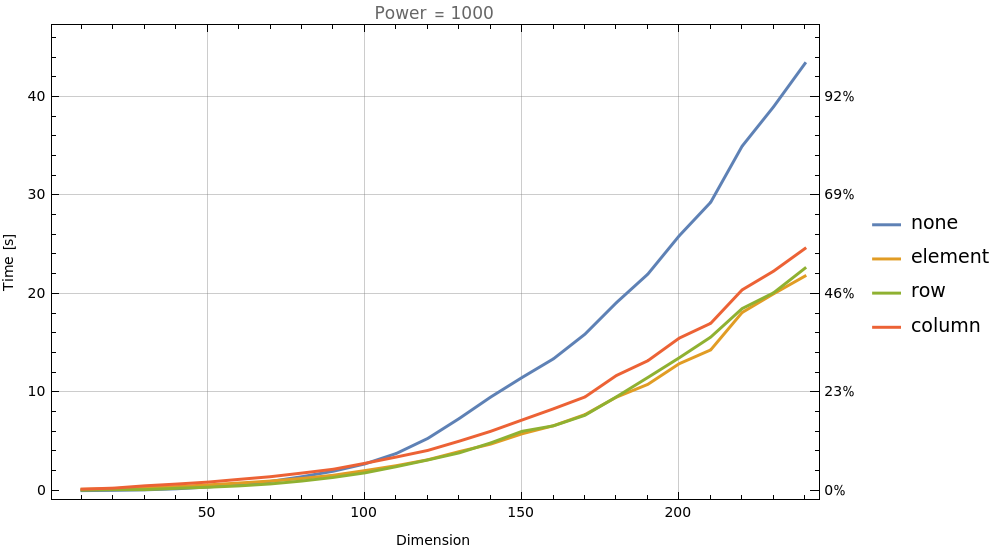
\includegraphics[width=0.75\textwidth]{images/dimension_small.png}
        \caption{Benchmarking for different forms of parallelism over matrix dimension, and a power of 1000.}
        \label{fig:small_dim}
    \end{figure}

    \begin{figure}[h]
        \centering
        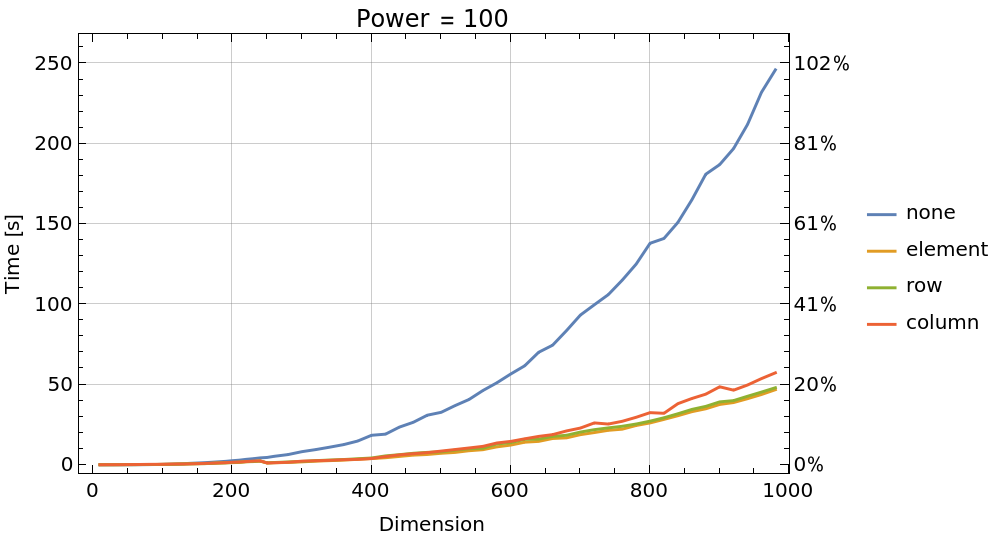
\includegraphics[width=0.75\textwidth]{images/dimension.png}
        \caption{Benchmarking for different forms of parallelism over matrix dimension, and a power of 100}
        \label{fig:med_dim}
    \end{figure}

    \begin{figure}[h]
        \centering
        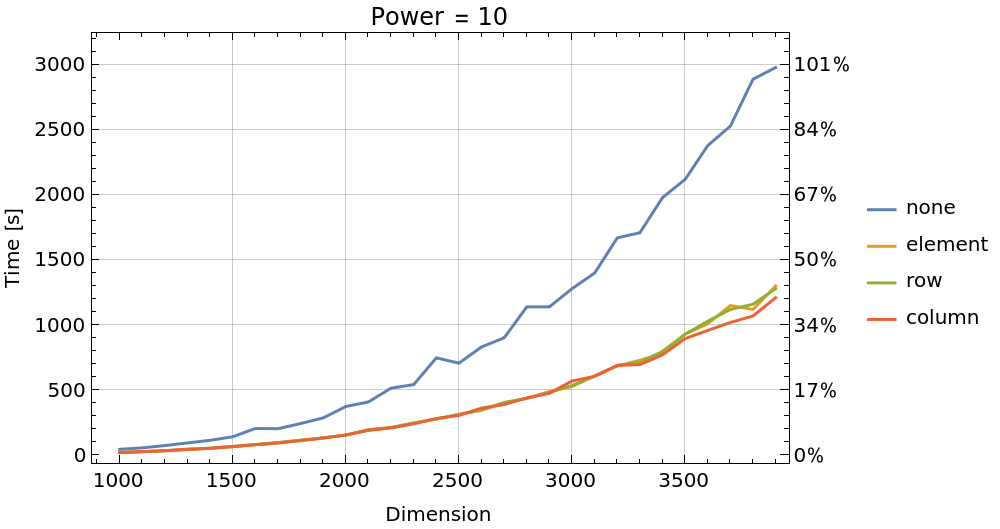
\includegraphics[width=0.75\textwidth]{images/big_dim.png}
        \caption{Benchmarking for different forms of parallelism over large matrix dimensions, and a power of 10}
        \label{fig:big_dim}
    \end{figure}

    Figure (\ref{fig:power}) shows how the execution time of the paralleized matrix power depends on the power to which the matrix is raised.

    \begin{figure}[h]
        \centering
        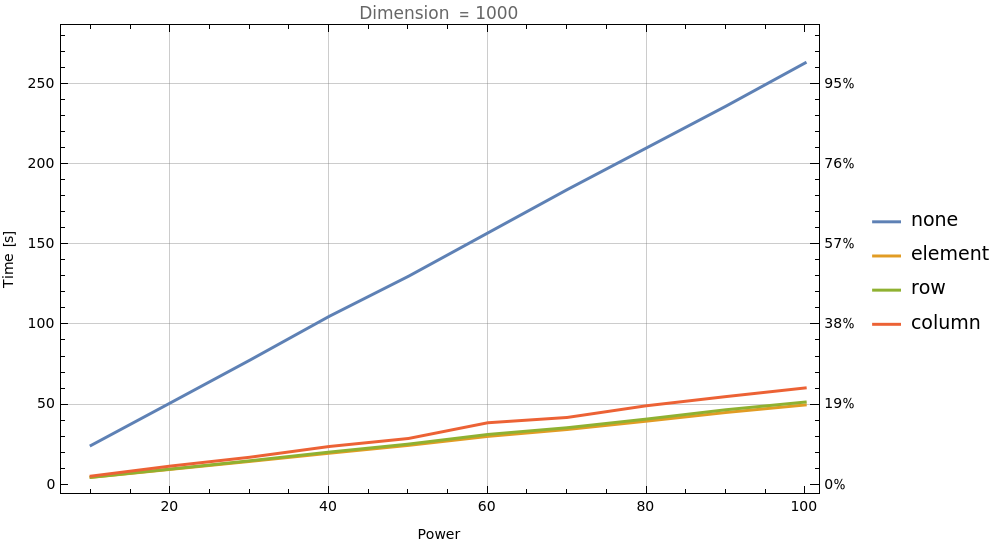
\includegraphics[width=0.75\textwidth]{images/power.png}
        \caption{Benchmarking for different forms of parallelism over large matrix dimensions, and a power of 10}
        \label{fig:power}
    \end{figure}

    The results in figures (\ref{fig:med_dim}, \ref{fig:power}, \ref{fig:small_dim}) were gathered on a machine with the specifications shown in table \ref{tbl:homeSpecs}, while the results in figure (\ref{fig:big_dim}) were gathered on a machine with specifications as show in table (\ref{tbl:officeSpecs}). 

    \begin{table}[h]
        \centering
        \begin{tabular}{|c||c|c|c|c|c|}
            \hline
            OS & Manjaro Linux \\
            \hline
            Kernel & Linux 6.6.30-2-MANJARO \\
            \hline
            Shell & bash 5.2.26 \\
            \hline
            CPU & 13th Gen Intel i7-13700K (24) @ 5.3GHz \\
            \hline
            GPU & NVIDIA GeForce RTX 3060 Ti Lite Hash Rate \\
            \hline
            Memory & 31.18GiB  \\
            \hline
            GPU Driver & NVIDIA 550.78 \\
            \hline
        \end{tabular}
        \caption{Different runtime complexities for different levels of paralleism in matrix multiplication.}
        \label{tbl:homeSpecs}
    \end{table}

    \begin{table}[h]
        \centering
        \begin{tabular}{|c||c|c|c|c|c|}
            \hline
            OS & Arch Linux \\
            \hline
            Kernel & Linux 6.6.30-2 \\
            \hline
            Shell & bash 5.2.26 \\
            \hline
            CPU & 6th Gen Intel i5-6500 (4) @ 3.2GHz \\
            \hline
            GPU & NVIDIA GeForce GTX 1660 Super \\
            \hline
            Memory & 16GiB  \\
            \hline
        \end{tabular}
        \caption{Different runtime complexities for different levels of paralleism in matrix multiplication.}
        \label{tbl:officeSpecs}
    \end{table}

\section{Discussion}

    
    While each figure could not more clearly suggest that using multiple threads to execute matrix multiplications is preferred when it comes to execution time, there are discrepancies between them.  Figure (\ref{fig:small_dim}) shows the parallel methods executing in only about 50\% of the time compared to the sequential version.  Compared to the over-50\% for large-dimensions (figure (\ref{fig:big_dim})) or even 80\% (wow!) reduction for medium-dimensions (figure \ref{fig:med_dim})

\section{Conclusion}

    \begin{itemize}
        \item a lot of applications take a long time because a lot of things need to be done
        \item these applications can benefit from parallelism via multithreading
        \item multithreading can be hard to implement
        \item sometimes it can be easier when the problem is embarissingly parallel
        \item new languages make parallelism trivial
        \item parallel implementation can save potentially massive amounts of time
        \item further parallelism and performance can be achieved with GPU programming like CUDA
    \end{itemize}

\end{document}